\documentclass[Report.tex]{subfiles}
\externaldocument[I-]{chapter_1_introduction.tex}
\externaldocument[D-]{chapter_3_discardMethod.tex}
\externaldocument[R-]{chapter_4_result.tex}
\externaldocument[C-]{chapter_5_conclusion.tex}
\externaldocument[RE-]{chapter_6_recognition.tex}

\begin{document}
\chapter{Method}
\label{chap:Method}
\section{Description}
The following section ,as mentioned in Section~\ref{subsec:Report Layout}, will present our methods. Bellow we present each component individually and the corresponding methods for them. A short description on what challenges have to
be solved for each component will be addressed first.

\section{Component: Text segmentation}
\label{Method:Text_segmentation}

\begin{flushleft}
  \textbf{Description} \\
In this part of the program, we want to be able to segment out text segments in the image. Afterwards we want to segment out lines and letter for further classification, see section \ref{subsec:Find_line} and \ref{subsec:Find_Symb} for reference. In this part we assume that the images have black text on white background, and it mostly consists of text.
\end{flushleft}

\begin{flushleft}
  \subsubsection{Approach: Simple Image Analysis Technics}
  Our approach here was inspired by this online blog \href{https://www.danvk.org/2015/01/07/finding-blocks-of-text-in-an-image-using-python-opencv-and-numpy.html}{Source}\cite{_finding_????}. We simplified the original approach to the following steps:
  \begin{enumerate}
    \item \textbf{Find Edges/Outliners of the image.}
    Initial idea is to use Canny, but we found Morphological Gradient to perform better. It indicates the contrast of the edges, so we can get better differences in some natural images (as long as the text and background are close to black and white respectively).
    \item \textbf{Otsu Thresholding.}
    We need our image to be a binary image. We simply use OpenCV Otsu algorithm to achieve it that.
    \item \textbf{Morphological Closing.}
    Since we want line segments we use Morphological Closing with large horizontal filter to merge as many horizontal letters together as possible.
    \item \textbf{Extract Regions}
    OpenCv FindContours was used to find the different text regions. We then exclude regions which are smaller than a selected threshold. The different region are return as coordinate of the different rectangular boxes.
  \end{enumerate}
\end{flushleft}

\section{Component: Preprocessing}
\label{Method:Preprocessing}
\begin{flushleft}
  \textbf{Description} \\
  Definition of preprocessing; the act of preparing the data for further use,
  in our case for classification. \par
  After the text segmentation we assume we have an image consisting of white text on black background. What remains for us to do is to segment out each character and format it to the right data type for the classifier. Hence we have 4 additional steps:
\end{flushleft}

\begin{flushleft}
  \textbf{Mini-steps}
  \begin{itemize}
    \item{Rotated text}
    \begin{itemize}
      \item{Our approach for character segmentation needs text rotated horizontally.}
    \end{itemize}
    \item{Line segmentation}
    \begin{itemize}
      \item{Our approach for character segmentation needs lines as input, as a sequence of lines on top of each other breaks the algorithm.}
    \end{itemize}
    \item{Character segmentation}
    \begin{itemize}
      \item{We need to segment each character because the classifier cannot distinguish several characters from one image.}
    \end{itemize}
    \item{Data formatting/casting}
    \begin{itemize}
      \item{The data we want to test a classifier on needs to match the data we trained our classifier with. Hence we need to format our data to the same format as the datasets. No need for a specific approach.}
    \end{itemize}
  \end{itemize}
\end{flushleft}

\subsection{Find rotation}
\begin{flushleft}
  \textbf{Approach: OpenCV minAreaRect() + CNN solution} \\
  This approach uses \href{https://en.wikipedia.org/wiki/Convex_hull}{convex hull}
  to find the convex hull of the text, and then
  \href{https://en.wikipedia.org/wiki/Rotating_calipers}{rotating calipers} to
  find the minimum area rectangle. \par
  cv.minAreaRect returns text rotated in one of following angles [0\textdegree, 90\textdegree, 180\textdegree, 270\textdegree], see Figure~\ref{fig:4angle_rot} for illustration. We will use a CNN to determine which of the angles is correct and then rotate it accordingly.
  To train the network we needed a dataset with the corresponding angles as labels, as we could not find one, we decided to create it ourself. 

  \begin{enumerate}
    \item \textbf{Binary image}
    For the Convex hull algorithm to work, the text segment and the background needs to be distinguishable. Convert image to a binary image using OpenCV threshold function and/or bitwise\textunderscore not to flip foreground and background colors.
    \item \textbf{cv.minAreaRect()}
    Feed our newly generated image to cv.minAreaRect.
    \item \textbf{calculate angle differences}
    From cv.minAreaRect() we can find the angle of the rectangle. From that we can calculate the angle of the potential rotated rectangle. 
    \item \textbf{Affine transform to rotate image}
    We use Affine transform to rotate the rectangle.
    \end{enumerate}
\end{flushleft}


\subsection{Find line}\label{subsec:Find_line}
After all the preprocessing done up to this point, we assume we have a segment of correctly rotated text. At this point it is enough to just use projection histogram. We basically sum number of active pixels in each row and end up with one dimensional array with same size as image height, one value for each row in input image.
E.g. [0 0 0 0 0 5 12 18 20 15 11 0 0 0 0 5 7 8..], this will mean there are some data (most likely text) between 5th and 10th row, and 15th  up to another line break. see fig \ref{fig:Project_histogram}
\begin{figure}[H]
  \centering
  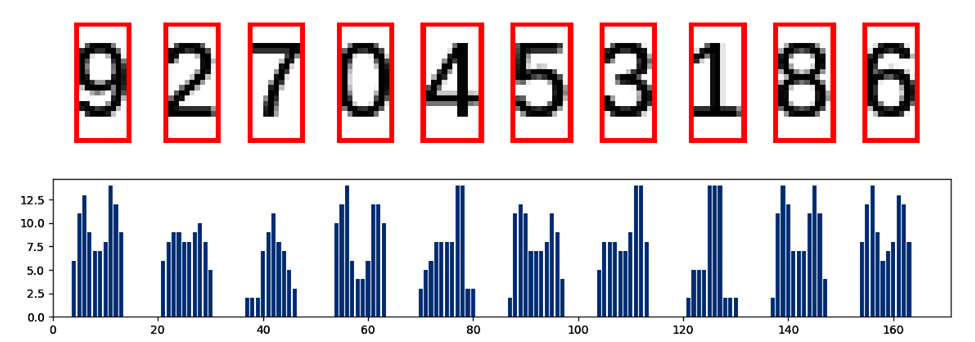
\includegraphics[width=\textwidth]{proj_histogram.png}
  \caption{Vertical project histogram, same applies to horizontal}
  \label{fig:Project_histogram}
\end{figure}


\subsection{Find Symbol/Letter Segmentation}\label{subsec:Find_Symb}
Letter segmentation was similar to Text Segmentation, section \ref{Method:Text_segmentation}. We added a few steps and kernel shape in the morphologic part. The additional step was to fill holes in the image, example like 8 and O can give multiple wrong contour. cv2.floodFill was used to solve this problem.
\begin{enumerate}
  \item Do threshold.
  \item Inverse the image since we work on black text on white background.
  \item Do morphological dilation with long vertical kernel, This is to include the dot in 'i'.
  \item Add a bolder around the line-image, that is separate elements from edge after previous step. This is to make cv2.floodFills work.
  \item Fill any holes, cv2.floodFills.
  \item Use cv2.FindContours
  \item Ignore element where contour size smaller than a threshold(half the letter size), to ignore ',','.' and other non letter element.
\end{enumerate}

\subsection{Data formatting/casting}\label{subsec:method:Data_formatting}
\todo[inline]{missing method:Data formatting/casting }
\begin{flushleft}
After we extracted single symbol from the line we have to feed it to the classificator. As we know our classificator accepts 28x28 grayscale images so we could simple resize the image to feed it, but this will more often than not yield poor results as the image will not follow the same convention images used to train the network did, execpt for the image size ofc. So we have to do some manipulations in order to make our image look more like images our CNN is good at recognizing. Lets take a look at some images from training sets: PICTURE FOLLOWS
As we can see the digit is centered and has about 4 pixels boarder around it. Furthermore it is not binary image with sharp edges, but rather smoothed out.  

The algorithm we found working best is described below:
First we find the dominant axis of the image using n = max(x, y), then we create new image with both axis equal $n + n//k$ where $k = 7$ as we found $\frac{28_{total-pixel}}{4_{border-pixel}} = 7$, then we paste our original character image in the center of newly created background image and only now resize it to 28x28 pixels. The resize operation will smooth the edges even though original digit may have been a binary image. Next we decided to out the noise by setting all pixels with intensity value under 50 to zero, and bring out the main shape of our character by setting all pixels with intensity value over 127 to 255.
And this gives us an image most likely to be correctly classified by our CNN.
\end{flushleft}

\section{Component: Classification}
\label{Method:Classification}
\begin{flushleft}
  \textbf{Description} \\
  For the classification component there where only 2 approaches we considered,
  Convolutional Neural Network (CNN), the architecture is illustration in
  Figure~\ref{fig:CNN_architecture}, and a Multilayer Perceptron (MLP or Deep
  neural network (DNN)), Figure~\ref{fig:neural_net2}. However the method we ended up choosing for the final result is CNN. In
  Section~\ref{sec:Discarded Method:Classification} we explain why we discarded
  the MLP approach. \par
\end{flushleft}

\begin{flushleft}
  \textbf{Convolutional Neural Network} \\
  The basic idea of a CNN is train some number of filters and then
  after the filters are trained, run the image which is now ``filtered'', through
  a fully connected network. The fully connected network will then try and
  classify based on the feature images from the convolution layers. \par
  A short description of key points of a CNN is presented in chapter \ref{chap:Recognition}. Below are the architecture and variable choices we have made for the CNN, 
\end{flushleft}

\begin{figure}[H]
  \centering
  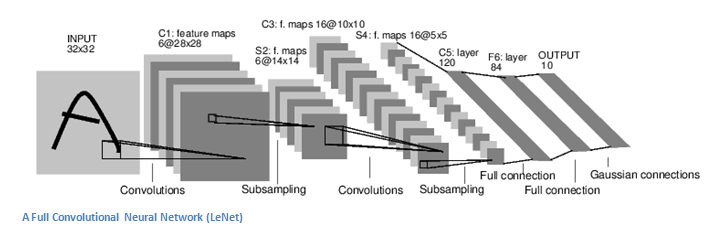
\includegraphics[height=4cm]{res/LeNet.png}
  \caption{Convolutional Neural network \href{https://adeshpande3.github.io/A-Beginner\%27s-Guide-To-Understanding-Convolutional-Neural-Networks/}{Source}}
  \label{fig:CNN_architecture}
\end{figure}

\todo[inline]{Architecture description should follow, choices of variables too \\
. \\
. \\
. \\
. \\
}


\section{Component: Datasets}
\label{Method:Datasets}

\todo[inline]{include only datasets we have used for the final software \\
Remove MNIST from this place, and moove it to chapter 3 discardMethod}

\subsection{Description}

\begin{flushleft}
  In order to learn our network to distinguish between the characters it needs training. Training is done by feeding images of known objects to the network (labeled data) and telling it how inaccurate it's prediction so that network can adjust it's weights accordingly. This type of training is called supervised training as we guide our network during training process.
  For network to get high accuracy of prediction a lot of labeled data is needed. Lucky for us datasets like MNIST exists, more info about it later.
\end{flushleft}

\begin{flushleft}
  \textbf{Limitation - proof-of-concept} \\
  As we have limited us to the digits and English alphabet, we will need labeled data for each of these [0..9] + 36 characters; divided into training, test and validation sets. As the concept of classifying only numbers vs all 36 characters does not differ that much, we will first see if we can solve the OCR problem with just numbers. Therefore we only need a dataset containing numbers at first. After that we can proceed our search for a dataset containing all the characters we need.
\end{flushleft}

\begin{flushleft}
  \textbf{Dataset} \\
  \textbf{MNIST} \\
  This is a dataset containing images of handwritten digits [0-9]. It has a training set of 60.000 examples and a test set of 10.000 examples. Training set is further divided into 55000 examples of actual training set, while 5000 images are treated as validation set (this number can be changed depending which interface we use to access MNIST data).
  MNIST dataset is compressed into 4 binary *.gz files, but we do not need to implement any readers/parsers ourself as tensorflow already has two we can choose between.
  (ref. reader to http://yann.lecun.com/exdb/mnist/).
\end{flushleft}
\end{document}
